% This is "sig-alternate.tex" V2.1 April 2013
% This file should be compiled with V2.5 of "sig-alternate.cls" May 2012
%
% This example file demonstrates the use of the 'sig-alternate.cls'
% V2.5 LaTeX2e document class file. It is for those submitting
% articles to ACM Conference Proceedings WHO DO NOT WISH TO
% STRICTLY ADHERE TO THE SIGS (PUBS-BOARD-ENDORSED) STYLE.
% The 'sig-alternate.cls' file will produce a similar-looking,
% albeit, 'tighter' paper resulting in, invariably, fewer pages.
%
% ----------------------------------------------------------------------------------------------------------------
% This .tex file (and associated .cls V2.5) produces:
%       1) The Permission Statement
%       2) The Conference (location) Info information
%       3) The Copyright Line with ACM data
%       4) NO page numbers
%
% as against the acm_proc_article-sp.cls file which
% DOES NOT produce 1) thru' 3) above.
%
% Using 'sig-alternate.cls' you have control, however, from within
% the source .tex file, over both the CopyrightYear
% (defaulted to 200X) and the ACM Copyright Data
% (defaulted to X-XXXXX-XX-X/XX/XX).
% e.g.
% \CopyrightYear{2007} will cause 2007 to appear in the copyright line.
% \crdata{0-12345-67-8/90/12} will cause 0-12345-67-8/90/12 to appear in the copyright line.
%
% ---------------------------------------------------------------------------------------------------------------
% This .tex source is an example which *does* use
% the .bib file (from which the .bbl file % is produced).
% REMEMBER HOWEVER: After having produced the .bbl file,
% and prior to final submission, you *NEED* to 'insert'
% your .bbl file into your source .tex file so as to provide
% ONE 'self-contained' source file.
%
% ================= IF YOU HAVE QUESTIONS =======================
% Questions regarding the SIGS styles, SIGS policies and
% procedures, Conferences etc. should be sent to
% Adrienne Griscti (griscti@acm.org)
%
% Technical questions _only_ to
% Gerald Murray (murray@hq.acm.org)
% ===============================================================
%
% For tracking purposes - this is V2.0 - May 2012

\documentclass{sig-alternate-05-2015}


\begin{document}

% Copyright
\setcopyright{acmcopyright}
%\setcopyright{acmlicensed}
%\setcopyright{rightsretained}
%\setcopyright{usgov}
%\setcopyright{usgovmixed}
%\setcopyright{cagov}
%\setcopyright{cagovmixed}


% DOI
\doi{10.475/123_4}

% ISBN
\isbn{123-4567-24-567/08/06}

%Conference
\conferenceinfo{PLDI '13}{June 16--19, 2013, Seattle, WA, USA}

\acmPrice{\$15.00}

%
% --- Author Metadata here ---
\conferenceinfo{CS265 Midway Checkin}{'97 El Paso, Texas USA}
%\CopyrightYear{2007} % Allows default copyright year (20XX) to be over-ridden - IF NEED BE.
%\crdata{0-12345-67-8/90/01}  % Allows default copyright data (0-89791-88-6/97/05) to be over-ridden - IF NEED BE.
% --- End of Author Metadata ---

\title{CS265 Midway Checkin 
%\titlenote{(Produces the permission block, and
%copyright information). For use with
%SIG-ALTERNATE.CLS. Supported by ACM.}
}
\subtitle{Optimizing Memory Allocation Between Memtable, Cache, and Bloom Filters
%\titlenote{A full version of this paper is available as
%\textit{Author's Guide to Preparing ACM SIG Proceedings Using
%\LaTeX$2_\epsilon$\ and BibTeX} at
%\texttt{www.acm.org/eaddress.htm}}
}
%
% You need the command \numberofauthors to handle the 'placement
% and alignment' of the authors beneath the title.
%
% For aesthetic reasons, we recommend 'three authors at a time'
% i.e. three 'name/affiliation blocks' be placed beneath the title.
%
% NOTE: You are NOT restricted in how many 'rows' of
% "name/affiliations" may appear. We just ask that you restrict
% the number of 'columns' to three.
%
% Because of the available 'opening page real-estate'
% we ask you to refrain from putting more than six authors
% (two rows with three columns) beneath the article title.
% More than six makes the first-page appear very cluttered indeed.
%
% Use the \alignauthor commands to handle the names
% and affiliations for an 'aesthetic maximum' of six authors.
% Add names, affiliations, addresses for
% the seventh etc. author(s) as the argument for the
% \additionalauthors command.
% These 'additional authors' will be output/set for you
% without further effort on your part as the last section in
% the body of your article BEFORE References or any Appendices.

\numberofauthors{3} %  in this sample file, there are a *total*
% of EIGHT authors. SIX appear on the 'first-page' (for formatting
% reasons) and the remaining two appear in the \additionalauthors section.
%
\author{
% You can go ahead and credit any number of authors here,
% e.g. one 'row of three' or two rows (consisting of one row of three
% and a second row of one, two or three).
%
% The command \alignauthor (no curly braces needed) should
% precede each author name, affiliation/snail-mail address and
% e-mail address. Additionally, tag each line of
% affiliation/address with \affaddr, and tag the
% e-mail address with \email.
%
% 1st. author
\alignauthor
Mali Akmanalp\\
       \affaddr{Harvard University}\\
       \email{mea590@g.harvard.edu}
% 2nd. author
\alignauthor
A. Sophie Hilgard\\
       \affaddr{Harvard University}\\
       \email{ash798@g.harvard.edu}
% 3rd. author
\alignauthor Andrew Ross\\
       \affaddr{Harvard University}\\
       \email{andrew\_ross@g.harvard.edu}}
% There's nothing stopping you putting the seventh, eighth, etc.
% author on the opening page (as the 'third row') but we ask,
% for aesthetic reasons that you place these 'additional authors'
% in the \additional authors block, viz.

\date{22 March 2017}
% Just remember to make sure that the TOTAL number of authors
% is the number that will appear on the first page PLUS the
% number that will appear in the \additionalauthors section.

\maketitle
\begin{abstract}
This paper provides a sample of a \LaTeX\ document which conforms,
somewhat loosely, to the formatting guidelines for
ACM SIG Proceedings. It is an {\em alternate} style which produces
a {\em tighter-looking} paper and was designed in response to
concerns expressed, by authors, over page-budgets.
It complements the document \textit{Author's (Alternate) Guide to
Preparing ACM SIG Proceedings Using \LaTeX$2_\epsilon$\ and Bib\TeX}.
This source file has been written with the intention of being
compiled under \LaTeX$2_\epsilon$\ and BibTeX.

The developers have tried to include every imaginable sort
of ``bells and whistles", such as a subtitle, footnotes on
title, subtitle and authors, as well as in the text, and
every optional component (e.g. Acknowledgments, Additional
Authors, Appendices), not to mention examples of
equations, theorems, tables and figures.

To make best use of this sample document, run it through \LaTeX\
and BibTeX, and compare this source code with the printed
output produced by the dvi file. A compiled PDF version
is available on the web page to help you with the
`look and feel'.
\end{abstract}


%
% The code below should be generated by the tool at
% http://dl.acm.org/ccs.cfm
% Please copy and paste the code instead of the example below. 
%
\begin{CCSXML}
<ccs2012>
<concept>
	<concept_id>10002951</concept_id>
	<concept_desc>Information systems</concept_desc>
	<concept_significance>500</concept_significance>
</concept>
<concept>
	<concept_id>10002951.10002952</concept_id>
	<concept_desc>Information systems~Data management systems</concept_desc>
	<concept_significance>500</concept_significance>
</concept>
<concept>
	<concept_id>10002951.10002952.10002953</concept_id>
	<concept_desc>Information systems~Database design and models</concept_desc>
	<concept_significance>300</concept_significance>
</concept>
</ccs2012>
\end{CCSXML}

\ccsdesc[500]{Information systems~Data management systems}
\ccsdesc[300]{Information systems~Database design and models}

%
% End generated code
%

%
%  Use this command to print the description
%
\printccsdesc

% We no longer use \terms command
%\terms{Theory}

\keywords{ACM proceedings; \LaTeX; text tagging}

\section{Introduction}
Tuning data systems is hard. Even for systems like key-value stores that only
support the most minimal API (\texttt{put} and \texttt{get}), the possibilities
are often overwhelming. The developers of RocksDB \cite{facebook:rocksdb}, a popular
and powerful key-value store, freely admit \cite{rocksdb-tuning-guide} that
``configuring RocksDB optimally is not trivial,'' and that ``even [they] as
RocksDB developers don't fully understand the effect of each configuration
change.'' Configurations must be optimized with respect to a given
\textit{workload}, which is rarely known in advance, although it is sometimes
roughly characterizable. There has been recent work \cite{monkey} in
determining the optimal memory allocation for bloom filters in terms of
worst-case analysis and with respect to a number of basic workloads, but
realistic key-value store workloads, which have been analyzed e.g. for Facebook
\cite{characterizing-memcached}, exhibit enormous complexity with respect to
time, skewness, and key repeatability.

Our goal is somewhat ambitious -- we seek to optimize not just bloom filter
memory allocation but memory allocation across the entire key-value store (to
cache, memtable, bloom filters, and possibly even fence pointers), and to do it
with respect to workloads we model as stochastic processes.

\section{Workloads}

Here are a number of basic workloads we will use to generate queries to
benchmark our key-value store, both in RocksDB and in Python simulations. For
the simpler ones, we will also attempt to predict performance and derive
optimal parameters analyitically.

\textbf{Uniform} queries will be drawn uniformly from keys $k \in
\{0,1,...,K\}$, where $K$ is a maximum key (that we explore varying). When we
draw a particular key $k_i$ for the first time, we will insert it into the
database as a write, and subsequently we will treat it as a lookup. Later we
will explore making a certain fraction of these queries into updates. The case
of uniformly distributed queries is often one in which the cache is unhelpful,
but in practice is highly unrealistic. Nevertheless, this is the scenario that
many analyses assume for calculations of big O complexity.

\textbf{Round-Robin} queries are drawn deterministically using $k_i = (i \mod
K)$, i.e. we iteratively draw each key in sequence, then repeat. This is also a
bad case for our key-value store in its default configuration; the fact that a
key has been recently written or read is actually a contraindication we will
access it again.

\textbf{80-20} queries (which are considered in \cite{monkey}) are drawn such
that 20\% of the most recently inserted keys constitute 80\% of the lookups.
This is a simple model we will be able to analyze analytically that exhibits
more realistic skew.

\textbf{Zipf} queries are distributed according to a Zipf or zeta distribution,
where the probability of a given key $k$ is $\propto \frac{1}{k^s}$, where $s
\in (1, \infty)$ describes the skewness of the distribution; in the limit
$s=1$, it is uniform with $K=\infty$. Zipf-distributed queries are considered
in \cite{art} as another simple proxy for realistically skewed queries.

\textbf{Discover-Decay} queries are distributed according to the following
stochastic process, inspired by the Chinese Restaurant process \cite{crp} but
with time decay: with every passing time increment $\Delta t \sim
\textrm{Expo}(\lambda_t)$, $n \sim \textrm{Pois}(\lambda_n)$ new keys are written to the
key-value store, which each have an inherent popularity $\theta_i \sim
\textrm{Beta}(a_\theta,b_\theta)$ with a random decay rate $\gamma_i \sim
\textrm{Beta}(a_\gamma,b_\gamma)$ that determines the exponential rate at which they
become less popular. The probability of drawing each $k_i$ is given by
$p(k_i,t) \propto \theta_i\gamma_i^{t-t_i}$, where $t$ is the current time and
$t_i$ is when the key was inserted. At each time step we sample $N$ keys from
$\textrm{Mult}(\{p(k_i,t)\})$. This stochastic process is somewhat arbitrary and we
hope to make it more realistic, but it does capture many of the essential
behaviors we know characterize key-value stores: new keys are constantly
inserted, some keys are much more popular than others, and the popularity of
most keys decays over time. The nonparametric nature of this stochastic process
may make inference difficult, and we also hope to enhance it to make it more
well-suited to realistic workloads (e.g. that exhibit daily periodicity), but
it seems much more able to simulate the richness of realistic queries than many
of the other models.

\section{Simulations}

We implemented a basic simulator of an LSM tree in Python \cite{lsmulator},
which simulates how an LSM tree with a variably sized cache, memtable, disk
layers, and bloom filters performs for an aribtrary sequence of queries. In
particular, we are able to simulate how often we are forced to access data on
disk (the main performance bottleneck for an LSM tree) and how often we can
respond with data in memory. So far, results suggest that the same LSM tree
architecture performs very differently under different query distributions
(Figure \ref{fig:sametree-diffqs}), and that different LSM tree architectures
perform very differently under the \textit{same} query distribution (Figure
\ref{fig:sameqs-difftree}). We are working on an optimization procedure to find
the best architecture for a given set of queries.

\begin{figure}[!htb]
\begin{center}
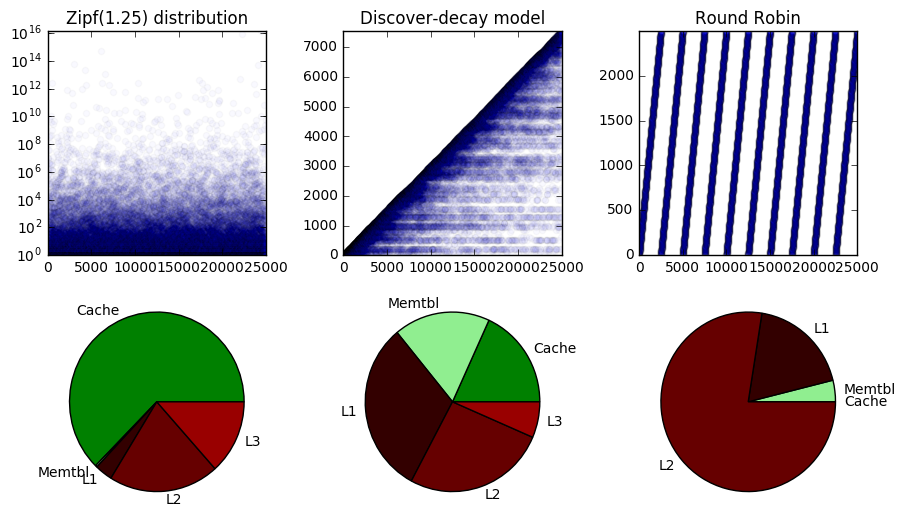
\includegraphics[width=9cm]{sametree-diffqs.png}
\end{center}
\caption{The same LSM tree architecture (a 25-element cache, 100-element
memtable, 5x layer ratio, and 10-bit bloom filters with 5 hash functions)
performs very differently for different query distributions. Memtable and cache
hits (in green) are fast, whereas accesses to the layers (in red) are slow. For
the Zipf workload, the cache is much more useful than the memtable, while the
situations are reversed for the Round-Robin workload. Both are useful in the
discover-decay case.}
\label{fig:sametree-diffqs}
\end{figure}

\begin{figure}[!htb]
\begin{center}
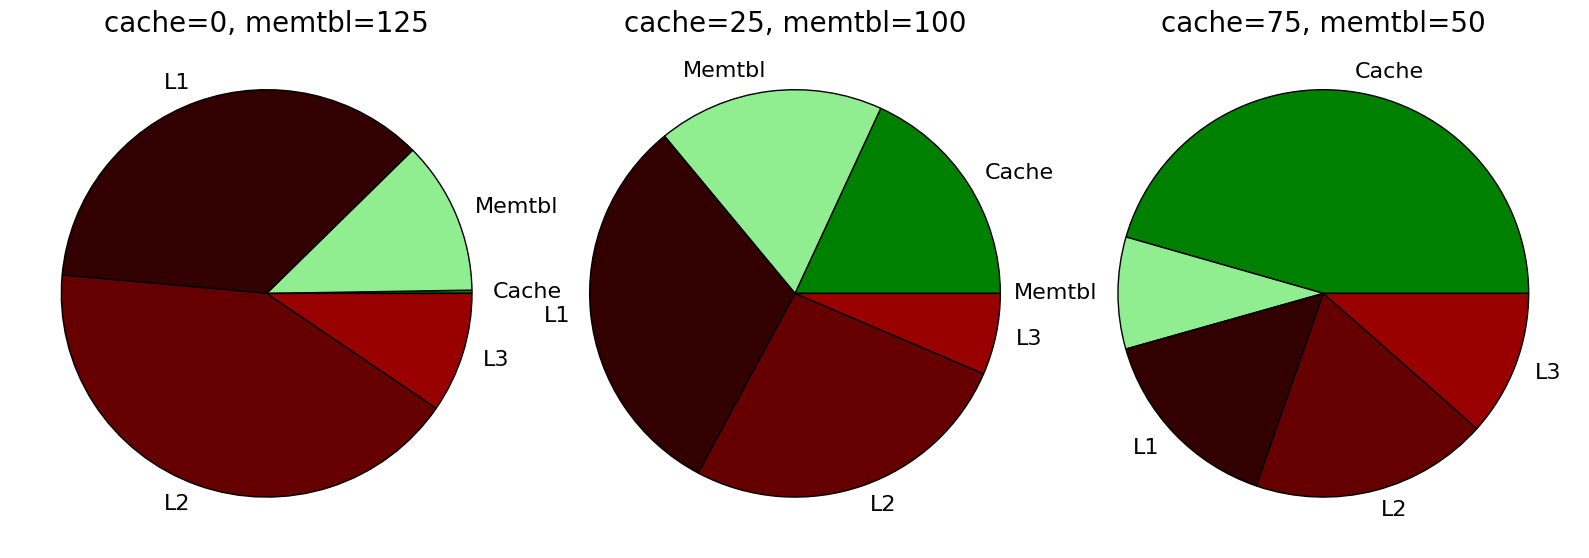
\includegraphics[width=9cm]{sameqs-difftree.png}
\end{center}
\caption{Performance results for different LSM tree architectures on the
discover-decay workload. Note that for this time-dependent workload, both the
cache and the memtable are useful, but finding the best ratio may require
optimization.}
\label{fig:sameqs-difftree}
\end{figure}

\section{Modeling}
\subsection{Uniform}
Assume \\
$n_t$ items in total DB \\
$n_c$ items that fit in cache\\
$n_m$ items that fit in memtable\\
$R$ ratio between layers of LSM tree such that \\
$L1 = R * n_m$ \\
$L2 = R^2 * n_m \dots$ \\ 

We can solve for $j$ the total number of layers required to store all the data: \\
$$n_m * \frac{1-R^j}{1-R} = n_t$$
$$j = \frac{log(1-n_t*\frac{1-R}{n_m})}{log R}$$

The average cost of a write remains the same as for the basic LSM tree case:
$$
\textrm{log}_{R} \frac{n_t}{n_m}
$$

The average cost of a read, we consider probabilistically over all possible locations of the read item, assuming a random distribution of reads: \\
Probability that read is in memtable:
$$\frac{n_m}{n_t}  = p(mt)$$\\
Probability that read is in cache:
$$\frac{n_c}{n_t} = p(cache)$$ \\
Probability that read is in L1 but not in cache
$$ \frac{n_m * R - \frac{n_m * R}{n_m * \frac{1-(R^j-1)}{1-R}} * n_c}{n_t}  = p(L1)$$\\
Where the numerator is the number of items that are in the first layer $$n_m * R$$ minus the proportion of items from that layer that are probabilistically in the cache already $$\frac{n_m * R}{n_m * \frac{1-(R^j-1)}{1-R}} * n_c$$
Probability that read is in $L_i$ generally but not in cache
$$ \frac{n_m * R^i - \frac{n_m * R^i}{n_m * \frac{1-(R^j-1)}{1-R}} * n_c}{n_t}  = p(L_i)$$\\
%Where the numerator is the number of items that are in the first layer $$n_m * R$$ minus the proportion of items from that layer that are probabilistically in the cache already $$\frac{n_m * R}{n_m * \frac{1-(R^j-1)}{1-R}} * n_c$$
Where here the $R^j -1$ comes from the fact that items already in memtable (L0) are not allowed to occupy the cache.

Expected cost of read:
$$E[C] = p(mt) * 0  + p(cache) * 0 + \sum_{i=1}^j p(L_i) * i$$
$$= \sum_{i=1}^j \frac{n_m * R^i - \frac{n_m * R^i}{n_m * \frac{1-(R^j-1)}{1-R}} * n_c}{n_t}  * i$$

\subsection{Skewed Reads (80-20)}

Now consider the case for skewed reads, where we say $d_{hf}$ ($d_{lf}$) percent of the data receives $r_{hf}$ ($r_{lf}$) percent of the reads (where $d_{hf} + d_{lf} = 1$ and $r_{hf} + r_{lf} = 1$). On average, we can assume that the cache contains $r_{hf} * n_c$ items from $d_{hf} * n_t$ and $r_{lf} * n_c$ items from $d_{lf} * n$. Then the expected cost of a read is dependent on whether the data item being read is in $d_{hf} * n_t$ or $d_{lf} * n$ as the probability of a cache hit varies.\\ \\
Concretely, consider where we have 3 levels and 800 total items with a cache of size 10 and a ratio of 2  (for L0=100, L1 = 200, L2 = 400 items), with $d_{hf} = .2$ and $d_{lf} = .8$ and $r_{hf}$ = .8 and $r_{lf}$ = .2. Then the cache on average contains 8 items from $d_{hf} * n$ and 2 items from $d_{lf}*n$. If we execute a read on one of the 200 items in $d_{hf}$, then, there is a $\frac{8}{200}$ chance that that item is in the cache. If we execute a read on one of the $200*\frac{1}{4} = 50$ items of  $d_{hf} * n_t$ in L1, we expect that $\frac{2}{6} * 8$ of those items would have actually been found already in cache, as this level contains $\frac{2}{6}$ of all of the items not in the memtable. Then the probability that a read is found in L1 is the proportion of the $d_{hf} * n_t = 160$ items that will reside in L1 but not in the cache, which is $\frac{40 - \frac{2}{6} * 8}{160}$. \\ \\
For data in $d_{hf} * n$, \\ \\
Probability that read is in memtable:
$$\frac{n_m*d_{hf}}{d_{hf} *n_t}  = p(mt_{hf})$$\\
Probability that read is in cache:
$$\frac{r_{hf} * n_c}{d_{hf} * n_t} = p(cache_{hf})$$ \\
Probability that read is in $L_i$ but not in cache:
$$ \frac{n_m * R^{i}*d_{hf} - \frac{n_m * R^{i}}{n_m * \frac{1-(R^j-1)}{1-R}} * r_{hf} * n_c}{d_{hf} * n_t}  = p(Li_{hf})$$ \\
Expected cost of read on item in $d_{hf}$:
$$E[C_{hf}]= p(mt_{hf}) * 0  + p(cache_{hf}) * 0 + \sum_{i=1}^j p(Li_{hf}) * i$$
$$ = \sum_{i=1}^j \frac{n_m * R^{i}*d_{hf} - \frac{n_m * R^{i}}{n_m * \frac{1-(R^j-1)}{1-R}} * r_{hf} * n_c}{d_{hf} * n_t}  * i$$

The expected cost of a read on an item in $d_{lf}$ can be enumerated analogously, and we combine the expectation of reads in $d_{hf}$ and $d_{lf}$ as: \\
Expected cost of read = $r_{hf} * E[C_{hf}] + r_{lf} * E[C_{lf}]$ \\ \\
%We can also define $r_{lf}$ in terms of $r_{hf}$ as $r_{hf} - 1$ and  $d_{lf}$ in terms of $d_{hf}$ as $d_{hf} - 1$ . (Doing this will make the effect that moving these parameters in one direction or the other has more obvious in the total overall formula.)
\subsection{Bloom Filters}

For a Bloom filter of $k$ bits with $h$ independent hash functions $h_1, h_2,...h_h$, the probability that a given bit is still set to 0 after inserting $n$ keys is 
$$
(1 - \frac{1}{k})^{n*h}
$$
Then the probability of a false positive is 
$$
(1- (1 - \frac{1}{k})^{n*h})^h \approx (1 - e^{-hn/k})^h
$$

We can minimize this over $h$ to find the optimal number of hash functions, which is $h = \mathrm{ln}(2) * \frac{k}{n}$. Assuming that this is the number of hash functions $h$ we will use, the probability of a false positive as a function of the number of bits is then 
$$
(1 - e^{-\mathrm{ln}(2)*k/n*n/k})^{\mathrm{ln}(2) * \frac{k}{n}} = (\frac{1}{2}) ^ {\mathrm{ln}(2) * \frac{k}{n}} \approx (.6185) ^  {\frac{k}{n}}
$$

For an item in any any level $L_i$ of the LSM tree with $i \geq 2$ we can reduce the expected cost of accessing that item from $i$ by the number of Bloom filter negatives at any level $j<i$. \\ \\
Then the expected cost of accessing an item at $L_i$ is  $$\sum_{j=1}^{i-1} p(fp_j) * 1 + 1$$
Where $p(fp_j)$ is the probability of a false positive for that key at level $j$ and 1 is the cost of actually accessing the item at level $i$ assuming fence pointers that lead us to the correct page.

\subsection{Variable Cache Size, Constant Number of Layers}
To analyze a variable cache/memtable allocation with a given memory size $n_v$, we first consider the simplification of assuming a constant layer structure. Of course, in general a larger memtable will allow for larger layers, affecting both read and write performance. Let $n_l$ be the size of the first layer when $n_v = n_m$ (all memtable) and $n_c =n_v - n_m$.\\ \\
\textbf{Uniform Case:} \\
%if we assume some fixed base layer size $n_l$, which is the size of the memtable if it exists.
Consider the formula used earlier:
$$
p(mt) * 0  + p(cache) * 0 + \sum_{i=1}^j p(L_i) * i 
$$

In the extreme case where $n_m=0$ (\textbf{no memtable}), the formula in the numerator of the sum simplifies to be over $n$ the total number of items, as there is no memtable layer and the probability of the first layer now has a cost of 1. However, we now have to add a number of items to each level of the tree that sum to the amount that were in L0. We add them as a geometric series per layer to maintain the structure
$$
\sum_{i=i}^{j} \frac{(n_l) * R^{i} + \frac{(n_l) * R^{i}}{n_t} * n_v - \frac{(n_l) * R^{i}}{n_t} * n_v}{n_t} * (i)
$$
The two latter terms cancel and we are left with
$$
\sum_{i=1}^j \frac{(n_l) * R^i}{n_t} * i 
$$
In the extreme case of \textbf{no cache}, 
$$
\sum_{i=1}^j \frac{(n_l) * R^i}{n_t} * i 
$$
And we can see that this is in fact the same result as the no memtable case. \\ \\
In general, for any selection of $n_m$ and $n_c$ we have
\begin{multline}
\sum_{i=1}^j \frac{(n_l) * R^i - \frac{(n_l) * R^i}{(n_l) * \frac{1-(R^j-1)}{1-R}} * (n_v-n_m)}{n_t} \\+
\frac{\frac{(n_l) * R^i}{(n_l) * \frac{1-(R^j-1)}{1-R}} * (n_v-n_m)}{n_t} * i 
\end{multline}
and so with a random workload, the choice is irrelevant \textit{assuming a constant number of layers}. In actuality, with a larger memtable we will be able to decrease the total number of layers needed. \\
\\
\textbf{Skewed Reads (80-20) Case:}\\
Now consider the case for skewed reads, where we say $d_{hf}$ ($d_{lf}$) percent of the data receives $r_{hf}$ ($r_{lf}$) percent of the reads (where $d_{hf} + d_{lf} = 1$ and $r_{hf} + r_{lf} = 1$). On average, we can assume that the cache contains $r_{hf} * n_c$ items from $d_{hf} * n_t$ and $r_{lf} * n_c$ items from $d_{lf} * n$. \\ \\
In the extreme case of \textbf{no cache}, the result will be as above. \\ \\
In the extreme case of \textbf{no memtable}, the expected cost of a read is dependent on whether the data item being read is in $d_{hf} * n_t$ or $d_{lf} * n$ as the probability of a cache hit varies.\\
For data in $d_{hf} * n$, \\ \\
Probability that read is in cache:
$$\frac{r_{hf} * n_c}{d_{hf} * n_t} = p(cache_{hf})$$ \\
Probability that read is in $L_i$ but not in cache: 
\begin{multline}
\frac{n_l * R^{i}*d_{hf} - \frac{n_l * R^{i}}{n_t} * r_{hf} * (n_v)}{d_{hf} * n_t} \\+ \frac{\frac{n_l * R^{i}}{n_t} *d_{hf} *(n_v)}{d_{hf} * n_t}  \\= \frac{n_l * R^{i}*d_{hf}+ \frac{n_l * R^{i}}{n_t} * (d_{hf}-r_{hf})* n_v}{d_{hf} * n_t} = p(Li_{hf}) 
\end{multline} \\
Expected cost of read on item in $d_{hf}$: \\
$$E[C_{hf}]= p(cache_{hf}) * 0 + \sum_{i=1}^j p(Li_{hf}) * i$$\\
$$
= \sum_{i=1}^j \frac{n_l * R^{i}*d_{hf}+ \frac{n_l * R^{i}}{n_t} * (d_{hf}-r_{hf})* n_v}{d_{hf} * n_t}  * i
$$ \\
From this equation we can see that the probability (and thus the expected cost) is increasing in $d_{hf}$ and decreasing in $r_{hf}$. This makes sense, as for many reads (high $r_{hf}$) on a small amount of data (low $d_{hf}$) we would expect frequent cache hits. \\ \\
For general memtable/cache allocation, probability that read is in $L_i$ but not in cache: 
\begin{multline}
\frac{n_l * R^{i}*d_{hf} - \frac{n_v * R^{i}}{n_l * \frac{1-(R^j-1)}{1-R}} * r_{hf} * (n_v - n_m)}{d_{hf} * n_t} \\+ \frac{\frac{n_v * R^{i}}{n_l * \frac{1-(R^j-1)}{1-R}} *d_{hf} *(n_v - n_m)}{d_{hf} * n_t}  = p(Li_{hf})
\end{multline}
%table showing expected effect of change in difft variables
\subsection{Allow Number of Layers to Vary with Memtable}
\subsection{Bloom Filter Allocation}

\section{Benchmarking}

So far, we've succeeded in getting basic benchmarks for RocksDB running and
identifying which configuration parameters to vary

\section{Conclusions}

%\end{document}  % This is where a 'short' article might terminate

%ACKNOWLEDGMENTS are optional
\section{Acknowledgments}


%
% The following two commands are all you need in the
% initial runs of your .tex file to
% produce the bibliography for the citations in your paper.
\bibliographystyle{abbrv}
\bibliography{sigproc}  % sigproc.bib is the name of the Bibliography in this case
% You must have a proper ".bib" file
%  and remember to run:
% latex bibtex latex latex
% to resolve all references
%
% ACM needs 'a single self-contained file'!
%
%APPENDICES are optional
%\balancecolumns
%\appendix
%%Appendix A
%\section{Headings in Appendices}
%The rules about hierarchical headings discussed above for
%the body of the article are different in the appendices.
%In the \textbf{appendix} environment, the command
%\textbf{section} is used to
%indicate the start of each Appendix, with alphabetic order
%designation (i.e. the first is A, the second B, etc.) and
%a title (if you include one).  So, if you need
%hierarchical structure
%\textit{within} an Appendix, start with \textbf{subsection} as the
%highest level. Here is an outline of the body of this
%document in Appendix-appropriate form:
%\subsection{Introduction}
%\subsection{The Body of the Paper}
%\subsubsection{Type Changes and  Special Characters}
%\subsubsection{Math Equations}
%\paragraph{Inline (In-text) Equations}
%\paragraph{Display Equations}
%\subsubsection{Citations}
%\subsubsection{Tables}
%\subsubsection{Figures}
%\subsubsection{Theorem-like Constructs}
%\subsubsection*{A Caveat for the \TeX\ Expert}
%\subsection{Conclusions}
%\subsection{Acknowledgments}
%\subsection{Additional Authors}
%This section is inserted by \LaTeX; you do not insert it.
%You just add the names and information in the
%\texttt{{\char'134}additionalauthors} command at the start
%of the document.

% This next section command marks the start of
% Appendix B, and does not continue the present hierarchy
%\section{More Help for the Hardy}
%The sig-alternate.cls file itself is chock-full of succinct
%and helpful comments.  If you consider yourself a moderately
%experienced to expert user of \LaTeX, you may find reading
%it useful but please remember not to change it.
%\balancecolumns % GM June 2007
% That's all folks!
\end{document}
